% Options for packages loaded elsewhere
\PassOptionsToPackage{unicode}{hyperref}
\PassOptionsToPackage{hyphens}{url}
%
\documentclass[
  11pt,
  ignorenonframetext,
]{beamer}
\usepackage{pgfpages}
\setbeamertemplate{caption}[numbered]
\setbeamertemplate{caption label separator}{: }
\setbeamercolor{caption name}{fg=normal text.fg}
\beamertemplatenavigationsymbolsempty
% Prevent slide breaks in the middle of a paragraph
\widowpenalties 1 10000
\raggedbottom
\setbeamertemplate{part page}{
  \centering
  \begin{beamercolorbox}[sep=16pt,center]{part title}
    \usebeamerfont{part title}\insertpart\par
  \end{beamercolorbox}
}
\setbeamertemplate{section page}{
  \centering
  \begin{beamercolorbox}[sep=12pt,center]{part title}
    \usebeamerfont{section title}\insertsection\par
  \end{beamercolorbox}
}
\setbeamertemplate{subsection page}{
  \centering
  \begin{beamercolorbox}[sep=8pt,center]{part title}
    \usebeamerfont{subsection title}\insertsubsection\par
  \end{beamercolorbox}
}
\AtBeginPart{
  \frame{\partpage}
}
\AtBeginSection{
  \ifbibliography
  \else
    \frame{\sectionpage}
  \fi
}
\AtBeginSubsection{
  \frame{\subsectionpage}
}
\usepackage{amsmath,amssymb}
\usepackage{lmodern}
\usepackage{iftex}
\ifPDFTeX
  \usepackage[T1]{fontenc}
  \usepackage[utf8]{inputenc}
  \usepackage{textcomp} % provide euro and other symbols
\else % if luatex or xetex
  \usepackage{unicode-math}
  \defaultfontfeatures{Scale=MatchLowercase}
  \defaultfontfeatures[\rmfamily]{Ligatures=TeX,Scale=1}
\fi
\usetheme[]{metropolis}
% Use upquote if available, for straight quotes in verbatim environments
\IfFileExists{upquote.sty}{\usepackage{upquote}}{}
\IfFileExists{microtype.sty}{% use microtype if available
  \usepackage[]{microtype}
  \UseMicrotypeSet[protrusion]{basicmath} % disable protrusion for tt fonts
}{}
\makeatletter
\@ifundefined{KOMAClassName}{% if non-KOMA class
  \IfFileExists{parskip.sty}{%
    \usepackage{parskip}
  }{% else
    \setlength{\parindent}{0pt}
    \setlength{\parskip}{6pt plus 2pt minus 1pt}}
}{% if KOMA class
  \KOMAoptions{parskip=half}}
\makeatother
\usepackage{xcolor}
\newif\ifbibliography
\usepackage{longtable,booktabs,array}
\usepackage{calc} % for calculating minipage widths
\usepackage{caption}
% Make caption package work with longtable
\makeatletter
\def\fnum@table{\tablename~\thetable}
\makeatother
\usepackage{graphicx}
\makeatletter
\def\maxwidth{\ifdim\Gin@nat@width>\linewidth\linewidth\else\Gin@nat@width\fi}
\def\maxheight{\ifdim\Gin@nat@height>\textheight\textheight\else\Gin@nat@height\fi}
\makeatother
% Scale images if necessary, so that they will not overflow the page
% margins by default, and it is still possible to overwrite the defaults
% using explicit options in \includegraphics[width, height, ...]{}
\setkeys{Gin}{width=\maxwidth,height=\maxheight,keepaspectratio}
% Set default figure placement to htbp
\makeatletter
\def\fps@figure{htbp}
\makeatother
\setlength{\emergencystretch}{3em} % prevent overfull lines
\providecommand{\tightlist}{%
  \setlength{\itemsep}{0pt}\setlength{\parskip}{0pt}}
\setcounter{secnumdepth}{-\maxdimen} % remove section numbering
\ifLuaTeX
  \usepackage{selnolig}  % disable illegal ligatures
\fi
\IfFileExists{bookmark.sty}{\usepackage{bookmark}}{\usepackage{hyperref}}
\IfFileExists{xurl.sty}{\usepackage{xurl}}{} % add URL line breaks if available
\urlstyle{same} % disable monospaced font for URLs
\hypersetup{
  pdftitle={Análisis de presencias con procesos de puntos},
  pdfauthor={Gerardo Martín},
  hidelinks,
  pdfcreator={LaTeX via pandoc}}

\title{Análisis de presencias con procesos de puntos}
\subtitle{Generalidades}
\author{Gerardo Martín}
\date{2022-06-29}

\begin{document}
\frame{\titlepage}

\hypertarget{introducciuxf3n}{%
\section{Introducción}\label{introducciuxf3n}}

\begin{frame}{¿Qué es un patrón de puntos?}
\protect\hypertarget{quuxe9-es-un-patruxf3n-de-puntos}{}
\begin{itemize}
\tightlist
\item
  Base de datos de cosas o eventos en espacio
\end{itemize}

\begin{figure}
\centering
\includegraphics{Figuras/Patrón-puntos.png}
\caption{Patrones de puntos de densidad variable. A la izquierda células
de mucosa gástrica en corte histológico. A la derecha, cúmulos de
galaxias (Baddeley et al.~2016).}
\end{figure}

\begin{itemize}
\tightlist
\item
  Densidad \(\rightarrow\) conteos/unidad espacial
\end{itemize}
\end{frame}

\begin{frame}{Tipos de puntos}
\protect\hypertarget{tipos-de-puntos}{}
Puntos pueden representar tipos de objetos

\begin{figure}
\centering
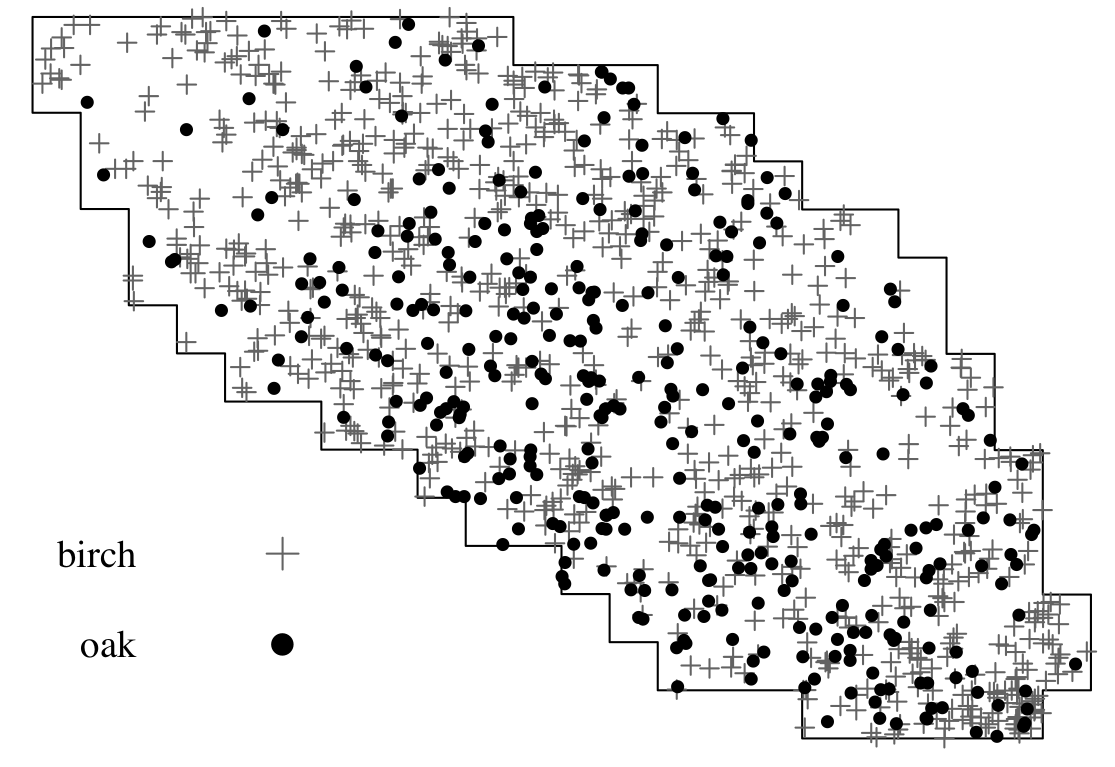
\includegraphics{Figuras/Tipos-puntos.png}
\caption{Ubicaciones de dos especie de árbol, abeto y roble, en la misma
parcela.}
\end{figure}
\end{frame}

\begin{frame}{Tipos de puntos}
\protect\hypertarget{tipos-de-puntos-1}{}
Puntos pueden representar mediciones

\begin{figure}
\centering
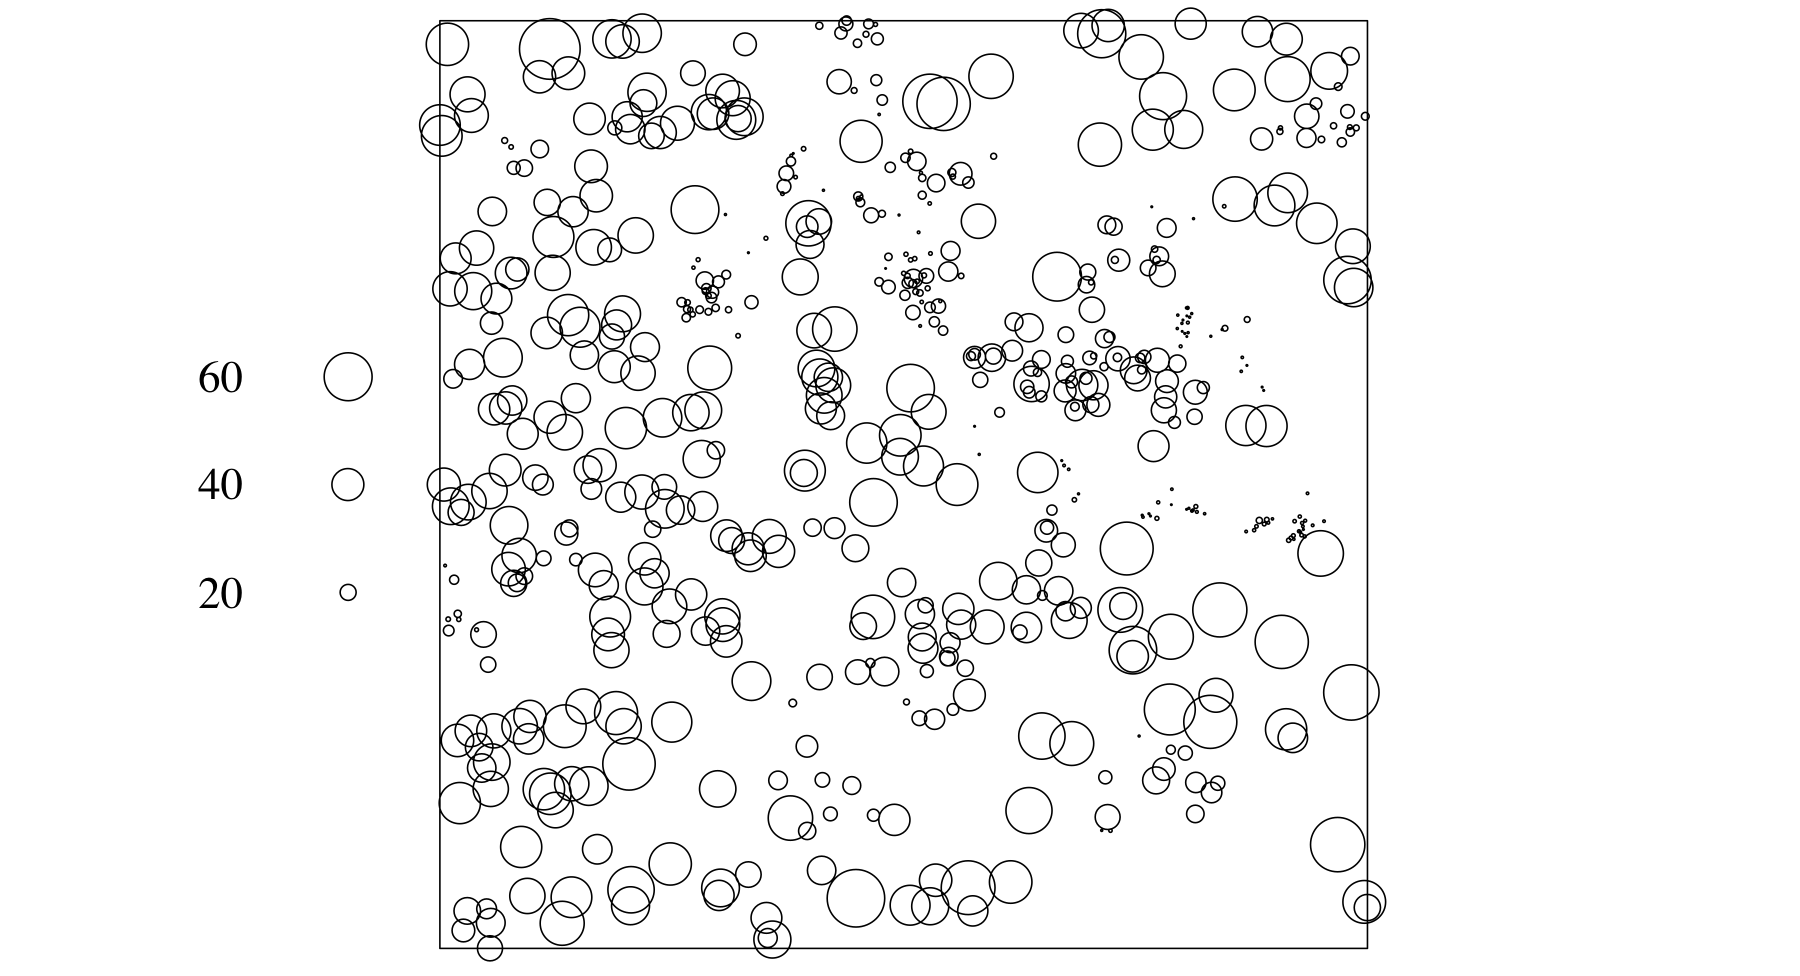
\includegraphics{Figuras/Tipos-puntos-med.png}
\caption{Ubicaciones de árboles con mediciones de diámetro.}
\end{figure}
\end{frame}

\begin{frame}{Tipos de puntos}
\protect\hypertarget{tipos-de-puntos-2}{}
Puntos pueden estar definidos en 1-4 dimensiones

\begin{figure}
\centering
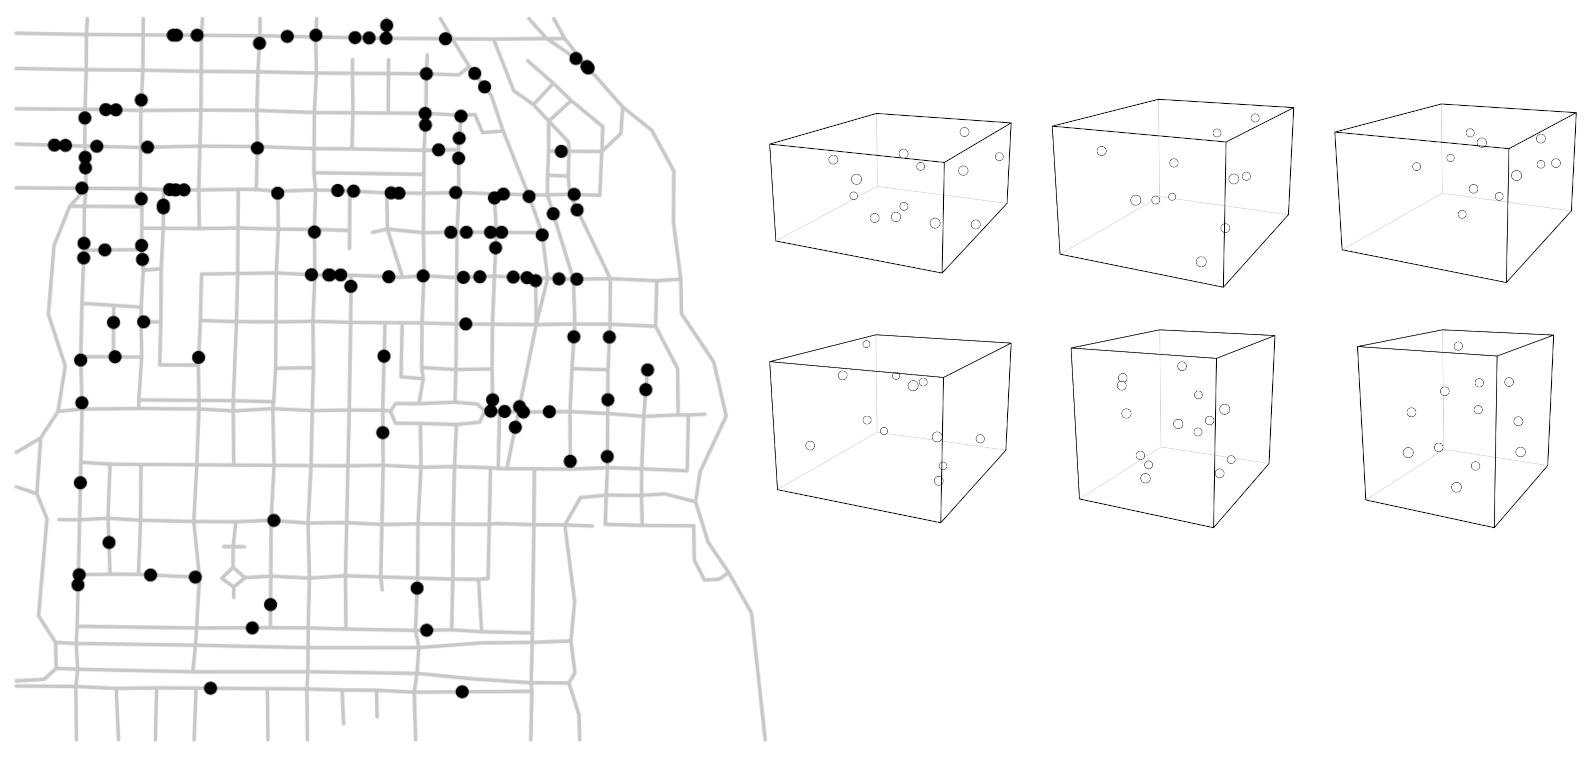
\includegraphics{Figuras/1-3D.png}
\caption{Ejemplos de procesos de puntos en 1 y 3 dimensiones}
\end{figure}
\end{frame}

\begin{frame}{Covariables}
\protect\hypertarget{covariables}{}
Los procesos de puntos pueden estar definidos en relación a covariables.

\begin{figure}
\centering
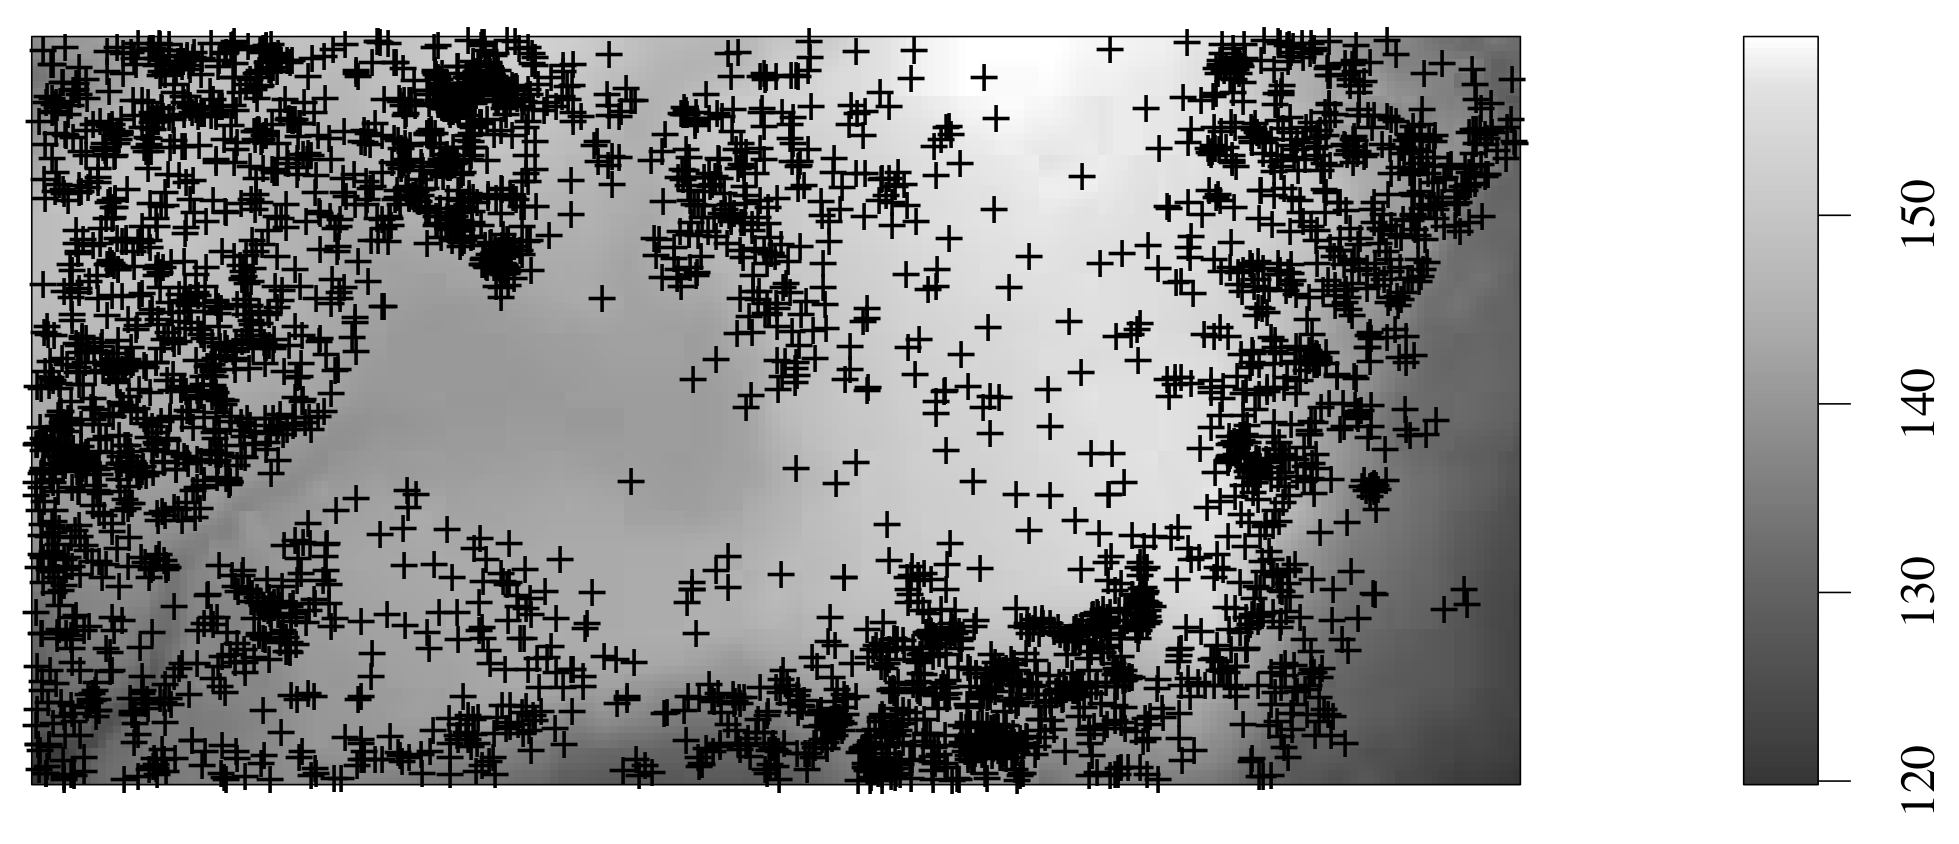
\includegraphics{Figuras/Covariables.png}
\caption{Datos de Beilschmiedia pendula sobre un modelo digital de
elevación.}
\end{figure}
\end{frame}

\begin{frame}{El modelado de procesos de puntos}
\protect\hypertarget{el-modelado-de-procesos-de-puntos}{}
\begin{itemize}
\item
  Estimar variación de densidad
\item
  Densidad = No.~puntos / unidad de área
\end{itemize}

\begin{figure}
\centering
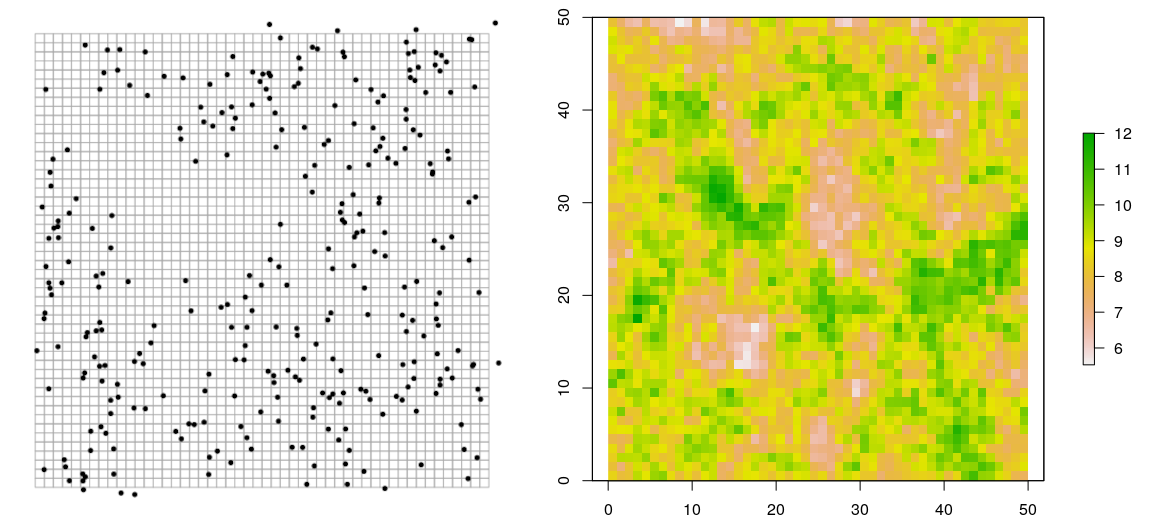
\includegraphics{Figuras/Conteos-estimacion.png}
\caption{Se analiza un patrón para predecir variación contínua.}
\end{figure}
\end{frame}

\begin{frame}{Procesos de puntos en ecología}
\protect\hypertarget{procesos-de-puntos-en-ecologuxeda}{}
\begin{itemize}
\item
  Datos más comunes \(\rightarrow\) sólo presencia
\item
  Colecciones de patrones de puntos
\end{itemize}

\begin{figure}
\centering

\includegraphics{Figuras/Repositorios.png}
\caption{Repositorios comunes de información de biodiversidad.}
\end{figure}
\end{frame}

\hypertarget{anuxe1lisis-de-procesos-de-puntos}{%
\section{Análisis de procesos de
puntos}\label{anuxe1lisis-de-procesos-de-puntos}}

\begin{frame}{Es un análisis regresión}
\protect\hypertarget{es-un-anuxe1lisis-regresiuxf3n}{}
\begin{itemize}
\item
  Medir relación entre \(x\) y \(y\) que son contínuas

  \begin{itemize}
  \tightlist
  \item
    ¿Cómo afecta \(x\) al promedio de \(y\)?
  \end{itemize}
\item
  \(x\) produce a \(y\)

  \begin{itemize}
  \tightlist
  \item
    \(x\) variable independiente
  \item
    \(y\) variable dependiente
  \end{itemize}
\end{itemize}
\end{frame}

\begin{frame}{Ejemplo - Datos contínuos}
\protect\hypertarget{ejemplo---datos-contuxednuos}{}
\begin{longtable}[]{@{}rr@{}}
\toprule()
x & y \\
\midrule()
\endhead
-0.5604756 & -1.2708822 \\
-0.2301775 & 0.0267062 \\
1.5587083 & 1.3120164 \\
0.0705084 & -0.2770342 \\
0.1292877 & -0.8223308 \\
1.7150650 & 1.6700373 \\
\bottomrule()
\end{longtable}
\end{frame}

\begin{frame}{Ejemplo - Gráfica de dispersión}
\protect\hypertarget{ejemplo---gruxe1fica-de-dispersiuxf3n}{}
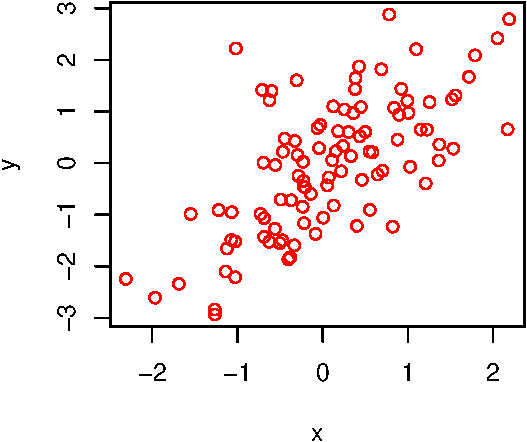
\includegraphics{Generalidades_files/figure-beamer/unnamed-chunk-2-1.pdf}
\end{frame}

\begin{frame}{Ejemplo - Regresión lineal}
\protect\hypertarget{ejemplo---regresiuxf3n-lineal}{}
\begin{itemize}
\tightlist
\item
  Regresión:
\end{itemize}

\[ y(x) = \alpha + \beta_1 x_1 + \dots + \beta_n x_n + \varepsilon\] -
\(x\) son las variables ambientales

\begin{itemize}
\item
  \(y\) es la intensidad por unidad de área
\item
  \(\alpha, \beta_i\) son los efectos de \(x\) sobre \(y\)
\item
  \(\varepsilon\) es el error, varianza de \(y\) que \(x\) no explica
\end{itemize}
\end{frame}

\begin{frame}{Ejemplo - La línea de regresión}
\protect\hypertarget{ejemplo---la-luxednea-de-regresiuxf3n}{}
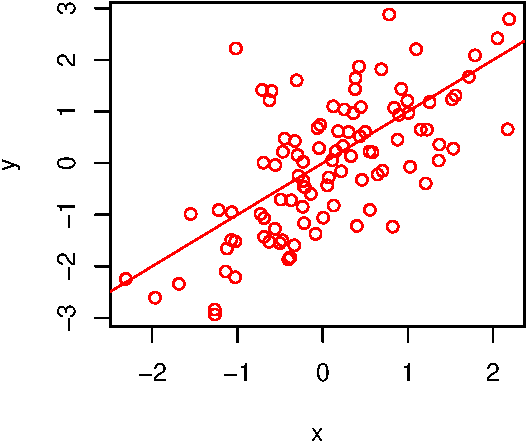
\includegraphics{Generalidades_files/figure-beamer/unnamed-chunk-3-1.pdf}
\end{frame}

\begin{frame}{Ejemplo - La ecuación}
\protect\hypertarget{ejemplo---la-ecuaciuxf3n}{}
\begin{itemize}
\item
  \(y = \alpha + \beta \times x\)
\item
  \(\alpha = 0\)
\item
  \(\beta = 1\)
\end{itemize}

\textbf{Regresión consiste en estimar todos los coeficientes para las
variables} \(x\).
\end{frame}

\begin{frame}{Diferencias entre regresión y PPs}
\protect\hypertarget{diferencias-entre-regresiuxf3n-y-pps}{}
\begin{itemize}
\item
  Regresión lineal simple

  \begin{itemize}
  \tightlist
  \item
    \(-\infty > y < \infty\), \(y \in \mathbb{R}\)
  \item
    \(y \approx \mathcal{N}\) (distribución Normal)
  \end{itemize}
\item
  Procesos de puntos

  \begin{itemize}
  \tightlist
  \item
    \(y > 0\), \(y \in \mathbb{Z}\)
  \item
    \(y \approx \mathcal{P}\) (distribución Poisson)
  \end{itemize}
\end{itemize}
\end{frame}

\begin{frame}{Diferencias entre regresión y PPs}
\protect\hypertarget{diferencias-entre-regresiuxf3n-y-pps-1}{}
Para que \(y >0\)

\begin{itemize}
\item
  Regresión lineal

  \begin{itemize}
  \tightlist
  \item
    \(y(x) = \alpha + \beta_1 x_1 + \dots\)
  \end{itemize}
\item
  Regresión log-lineal

  \begin{itemize}
  \tightlist
  \item
    \(\log y(x) = \alpha + \beta_1 x_1 + \dots\)
  \end{itemize}
\end{itemize}
\end{frame}

\begin{frame}{Relación con métodos populares}
\protect\hypertarget{relaciuxf3n-con-muxe9todos-populares}{}
\begin{itemize}
\item
  Equivalentes a MaxEnt

  \begin{itemize}
  \tightlist
  \item
    Sin Regularización
  \item
    \emph{Features} lineal y cuadrática
  \end{itemize}
\end{itemize}

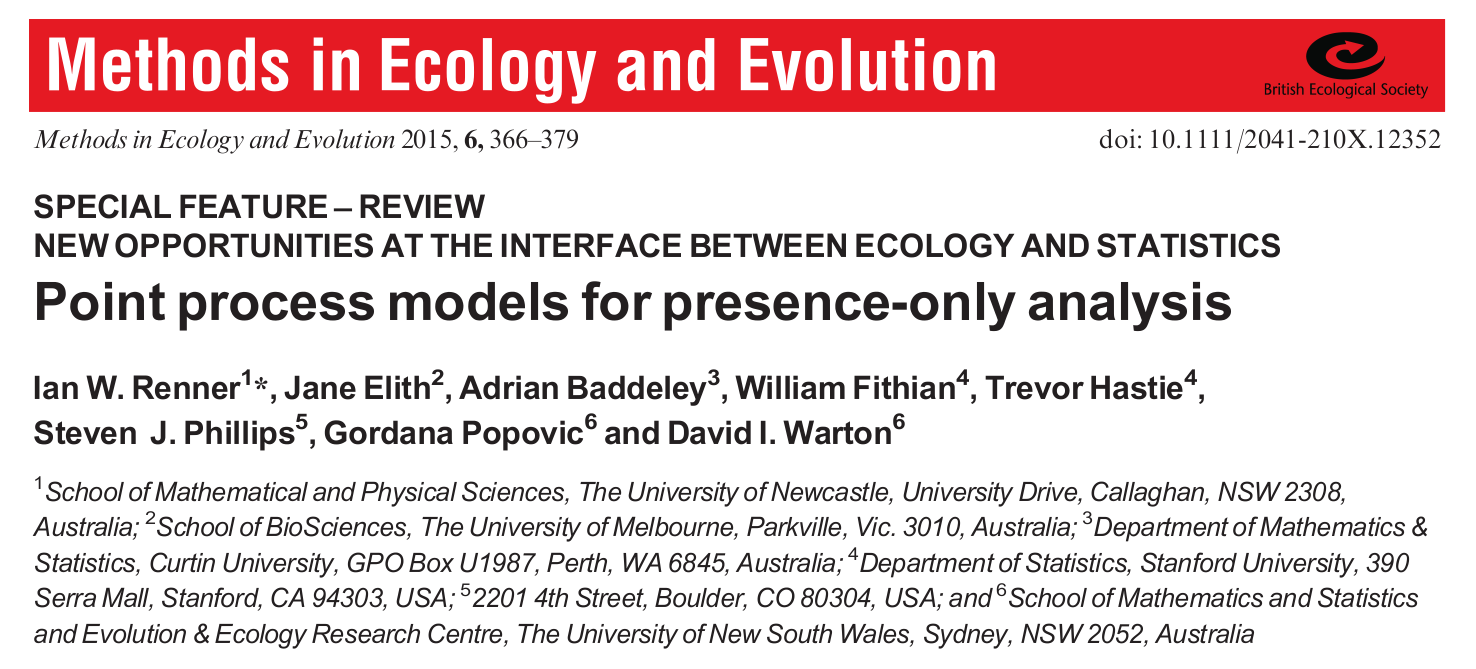
\includegraphics{Figuras/Renner.png}
\end{frame}

\begin{frame}{Relación con otros métodos}
\protect\hypertarget{relaciuxf3n-con-otros-muxe9todos}{}
\begin{itemize}
\item
  Regresión log-lineal

  \begin{itemize}
  \tightlist
  \item
    Logística
  \item
    Maxent
  \end{itemize}
\item
  Elipsoides (Martín et al.~2022)

  \begin{itemize}
  \tightlist
  \item
    Centroide existe en espacio
  \item
    Sin colinealidad
  \end{itemize}
\end{itemize}
\end{frame}

\begin{frame}{Relación con otros métodos}
\protect\hypertarget{relaciuxf3n-con-otros-muxe9todos-1}{}
Condiciones para equivalencia entre MPPs y envolturas


\includegraphics{Figuras/Discrep.png}
\end{frame}

\hypertarget{ventajas-y-desventajas}{%
\section{Ventajas y Desventajas}\label{ventajas-y-desventajas}}

\begin{frame}{Ventajas}
\protect\hypertarget{ventajas}{}
\begin{itemize}
\tightlist
\item
  Herramienta \emph{ad-hoc} para puntos
\item
  Transparencia
\item
  Herramientas exploratorias \(\rightarrow\) identificar variables
\item
  Estimación de efectos estadísticos
\item
  Tipos de puntos \(\rightarrow\) interacciones biológicas
\item
  Extensiones para modelar estructura espacial (maximizar utilidad de
  datos)
\item
  Herramientas diagnósticas
\end{itemize}
\end{frame}

\begin{frame}{Desventajas}
\protect\hypertarget{desventajas}{}
\begin{itemize}
\tightlist
\item
  Formateo
\item
  Difícil automatizar
\item
  Más programación
\item
  Selección de modelo laboriosa
\item
  Optimización puede ser difícil
\item
  Poco práctico para muchas especies
\end{itemize}
\end{frame}

\begin{frame}{Bibliografía básica}
\protect\hypertarget{bibliografuxeda-buxe1sica}{}
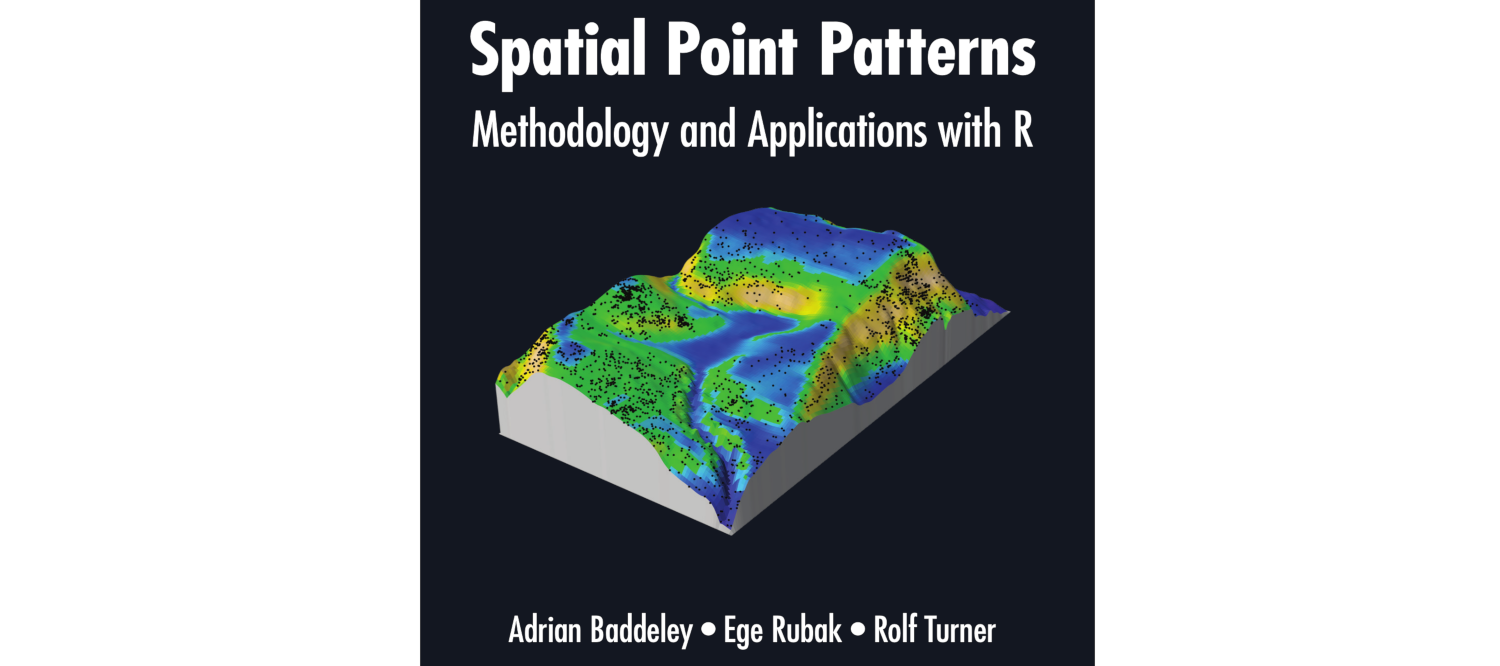
\includegraphics{Figuras/Spat-book.png}
\end{frame}

\end{document}
